\clearpage
\section{Supplementary figures}\label{app:suppfig}

\setcounter{figure}{0}
\renewcommand{\thefigure}{S\arabic{figure}}
\renewcommand{\theHfigure}{S\arabic{figure}}

Supplementary Figures~\ref{fig:tk}--\ref{fig:qcrej} show cases chosen by fixed rules with a fixed seed, not the
best-looking ones. The rules are stated in each legend; the inputs are listed in the code repository's storage
index.

\begin{figure}[htbp]
\centering
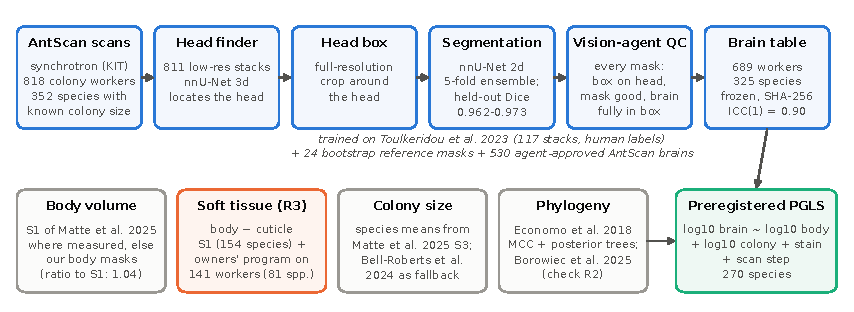
\includegraphics[width=0.9\textwidth]{figures/figS1_pipeline_schematic.pdf}
\caption[Measurement and analysis pipeline (schematic)]{\textbf{Measurement and analysis pipeline (schematic).}
AntScan synchrotron scans of colony workers pass through low-resolution brain localisation, a full-resolution head
box, the segmentation ensemble (nnU-Net 2d, 5 folds), vision-agent QC and the frozen brain table. Body volume, soft
tissue, colony size and the phylogeny enter the preregistered PGLS model~\eqref{eq:pgls}. Figure~\ref{fig:scan} shows
the same steps on real scans.}
\label{fig:schematic}
\end{figure}

\begin{figure}[htbp]
\centering
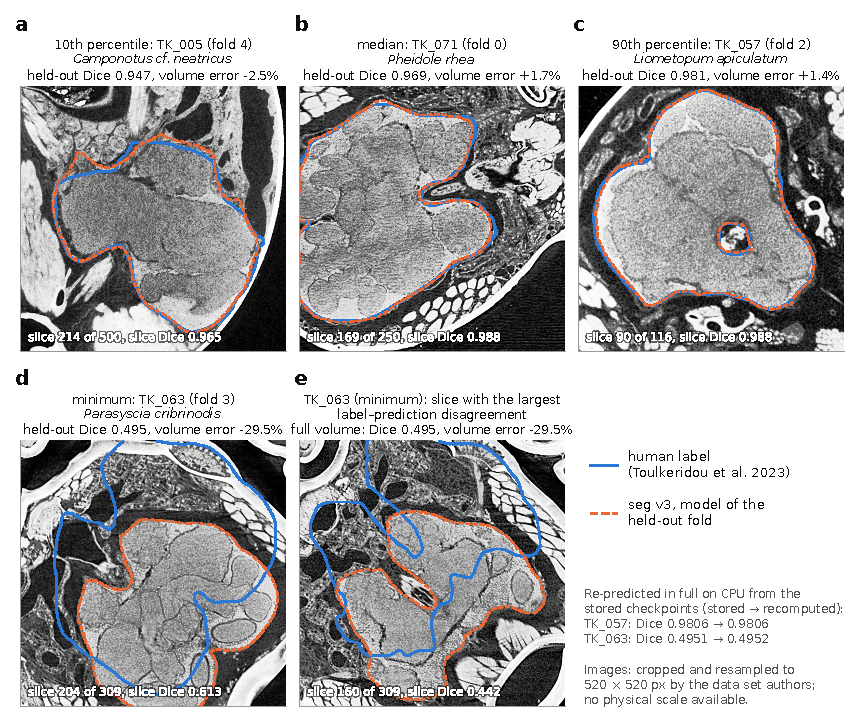
\includegraphics[width=0.86\textwidth]{figures/figS2_tk_heldout.pdf}
\caption[Segmentation model against human labels on held-out Toulkeridou cases]{\textbf{Segmentation model against
human labels on held-out Toulkeridou cases.} Four of the $117$ human-labelled stacks of \citet{toulkeridou2023} that were held out in
cross-validation. \emph{Selection rule:} the cases nearest the 10th, 50th and 90th percentile of per-case held-out
Dice (a--c) and the case with the lowest Dice (d--f). Each case was predicted by the segmentation model of the fold
whose validation set contains it; folds were split by species, so the species was not in training. Blue: human
label; orange, dashed: segmentation model of the held-out fold.
\textbf{(a--d)}~The slice with the largest labelled area. Titles give the held-out Dice and volume error of the full
volume; tiles give the Dice of the shown slice.
\textbf{(e)}~For the lowest case, the slice with the largest label--prediction disagreement.
\textbf{(f)}~The same slice with the human label moved by the rigid offset described below.
In the lowest case, the label in the deposited training archive is offset from its image by about
$115 \times 27$~pixels on every slice; moved back by this rigid shift, it outlines the brain (panel f; full-volume
Dice $0.812$ instead of $0.495$). The shifted label is still about $1.4$ times larger than the predicted brain, so the
deposited label was probably drawn on a differently cropped version of the image. A check of all $117$ held-out
reference labels (rigid-offset rule fixed before the check: shift $\geq 5$~px, Dice gain $\geq 0.10$, consistent
across slices) flagged only this stack. We kept it in Figure~\ref{fig:scan}d--e and Table~\ref{tab:S2}; without it
the median Dice is unchanged. Across the $117$ cases the median Dice was $0.969$, and $3$ cases were below $0.90$.
The dataset authors cropped and resampled the images to $520 \times 520$ pixels per slice, so no physical scale is
given.}
\label{fig:tk}
\end{figure}

\begin{figure}[htbp]
\centering
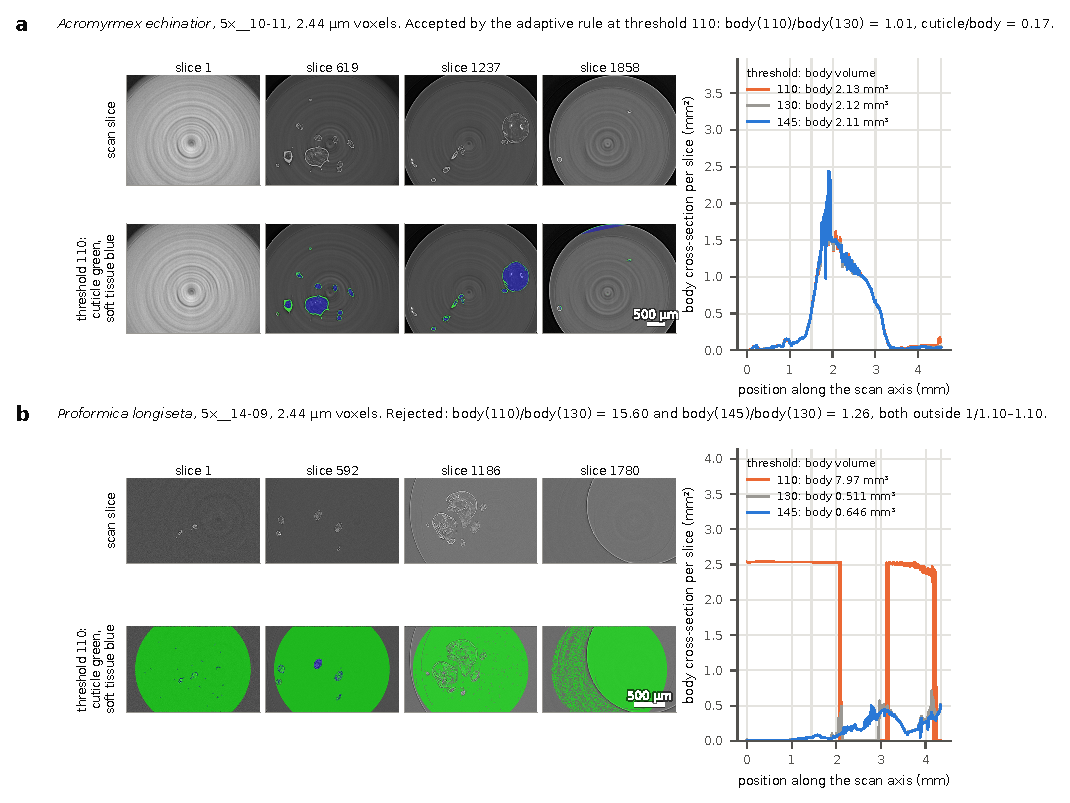
\includegraphics[width=\textwidth]{figures/figS3_cuticle_qc.pdf}
\caption[Body and cuticle segmentation by the owners' program, and the QC rule]{\textbf{Body and cuticle segmentation
by the owners' program, and the QC rule.} One specimen accepted and one rejected by the adaptive rule
(Section~\ref{sec:body}). \emph{Selection rule:} drawn at random (seed 20261116) from the $92$ specimens accepted at
threshold $110$ and from the $21$ specimens rejected with $\body{110}/\body{130} > 1.10$, the signature of a bright
mounting medium entering the mask. These $21$ are among the $37$ specimens for which neither threshold gave a stable
body volume; $7$ further specimens failed the cuticle/body limits. Left: the QC sheet written by our run of the
owners' program, with its tiles rearranged. The top row shows four evenly spaced slices of the processed range, and
the bottom row the segmentation at threshold $110$ (cuticle green, soft tissue blue). Right: body cross-section of
every sampled slice (every third slice) at thresholds $110$, $130$ and $145$, with the specimen's body volume at each
threshold; grey lines mark the slices shown on the left.
\textbf{(a)}~Accepted: the three thresholds give the same body ($\body{110}/\body{130} = 1.01$).
\textbf{(b)}~Rejected: at threshold $110$ the mounting medium fills the vial over long stretches of the stack, so
$\body{110}$ is $15.6$ times $\body{130}$; threshold $145$ also differs from $130$ by more than $10\%$.}
\label{fig:cuticle}
\end{figure}

\begin{figure}[htbp]
\centering
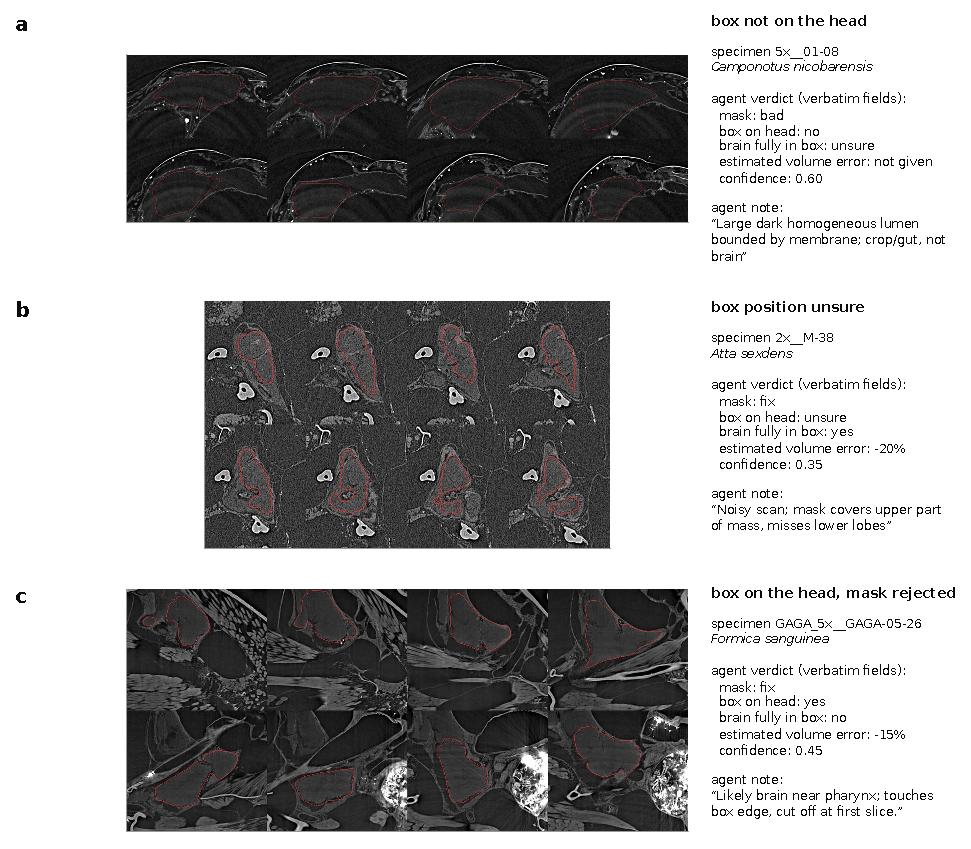
\includegraphics[width=0.92\textwidth]{figures/figS4_qc_rejections.pdf}
\caption[Masks rejected by the vision-agent QC]{\textbf{Masks rejected by the vision-agent QC.} Three masks from the
final QC round on masks of the segmentation ensemble in boxes from the final head finder: $268$ masks were reviewed, $124$ accepted and
$144$ rejected. The rejected masks fall into three categories by the agent's box verdict: box not on the head ($62$),
box position unsure ($45$) and box on the head but mask not good or brain not fully in the box ($37$).
\emph{Selection rule:} within each category, one mask was drawn at random (seed 20261116) among specimens absent from
the frozen table and with a non-empty mask ($20$, $25$ and $28$ eligible). Left: the contact sheet exactly as the
agent reviewed it: eight slices through the head box with the mask outline in red. Right: the verdict fields and the
agent's note, verbatim.
\textbf{(a)}~The agent judged the masked structure to be the crop or gut, not the brain.
\textbf{(b)}~The agent could not decide whether the box was on the head, and judged the mask incomplete.
\textbf{(c)}~The agent judged the box to be on the head but the brain to be cut off by a box face.}
\label{fig:qcrej}
\end{figure}
